\documentclass[14pt]{extbook}
\usepackage{multicol, enumerate, enumitem, hyperref, color, soul, setspace, parskip, fancyhdr} %General Packages
\usepackage{amssymb, amsthm, amsmath, latexsym, units, mathtools} %Math Packages
\everymath{\displaystyle} %All math in Display Style
% Packages with additional options
\usepackage[headsep=0.5cm,headheight=12pt, left=1 in,right= 1 in,top= 1 in,bottom= 1 in]{geometry}
\usepackage[usenames,dvipsnames]{xcolor}
\usepackage{dashrule}  % Package to use the command below to create lines between items
\newcommand{\litem}[1]{\item#1\hspace*{-1cm}\rule{\textwidth}{0.4pt}}
\pagestyle{fancy}
\lhead{Module6}
\chead{}
\rhead{Version C}
\lfoot{2107-1615}
\cfoot{}
\rfoot{test}
\begin{document}

\begin{enumerate}
\litem{
Construct the lowest-degree polynomial given the zeros below. Then, choose the intervals that contain the coefficients of the polynomial in the form $x^3+bx^2+cx+d$.\[ -5 + 4 i \text{ and } 1 \]\begin{enumerate}[label=\Alph*.]
\item \( b \in [0, 8], c \in [-9, -1], \text{ and } d \in [-1, 6] \)
\item \( b \in [0, 8], c \in [0, 10], \text{ and } d \in [-6, 2] \)
\item \( b \in [-14, -8], c \in [30, 39], \text{ and } d \in [40, 48] \)
\item \( b \in [7, 15], c \in [30, 39], \text{ and } d \in [-46, -29] \)
\item \( \text{None of the above.} \)

\end{enumerate} }
\litem{
Construct the lowest-degree polynomial given the zeros below. Then, choose the intervals that contain the coefficients of the polynomial in the form $ax^3+bx^2+cx+d$.\[ \frac{1}{4}, \frac{2}{3}, \text{ and } -7 \]\begin{enumerate}[label=\Alph*.]
\item \( a \in [3, 16], b \in [70, 76], c \in [-84, -73], \text{ and } d \in [-18, -11] \)
\item \( a \in [3, 16], b \in [92, 96], c \in [72, 87], \text{ and } d \in [8, 15] \)
\item \( a \in [3, 16], b \in [78, 85], c \in [-44, -33], \text{ and } d \in [-18, -11] \)
\item \( a \in [3, 16], b \in [70, 76], c \in [-84, -73], \text{ and } d \in [8, 15] \)
\item \( a \in [3, 16], b \in [-76, -67], c \in [-84, -73], \text{ and } d \in [-18, -11] \)

\end{enumerate} }
\litem{
Describe the zero behavior of the zero $x = 3$ of the polynomial below.\[ f(x) = -9(x - 6)^{5}(x + 6)^{4}(x + 3)^{11}(x - 3)^{8} \]\begin{enumerate}[label=\Alph*.]
\begin{multicols}{2}\item 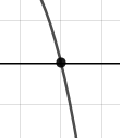
\includegraphics[width = 0.3\textwidth]{../Figures/polyZeroBehaviorAC.png}\item 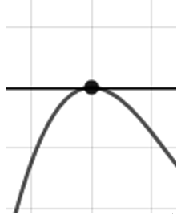
\includegraphics[width = 0.3\textwidth]{../Figures/polyZeroBehaviorBC.png}\item 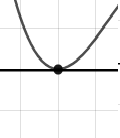
\includegraphics[width = 0.3\textwidth]{../Figures/polyZeroBehaviorCC.png}\item 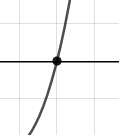
\includegraphics[width = 0.3\textwidth]{../Figures/polyZeroBehaviorDC.png}\end{multicols}\item None of the above.
\end{enumerate} }
\litem{
Describe the zero behavior of the zero $x = -8$ of the polynomial below.\[ f(x) = -8(x - 6)^{7}(x + 6)^{3}(x + 8)^{8}(x - 8)^{7} \]\begin{enumerate}[label=\Alph*.]
\begin{multicols}{2}\item 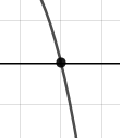
\includegraphics[width = 0.3\textwidth]{../Figures/polyZeroBehaviorCopyAC.png}\item 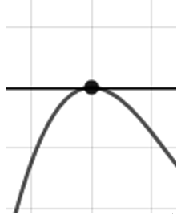
\includegraphics[width = 0.3\textwidth]{../Figures/polyZeroBehaviorCopyBC.png}\item 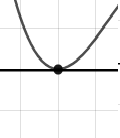
\includegraphics[width = 0.3\textwidth]{../Figures/polyZeroBehaviorCopyCC.png}\item 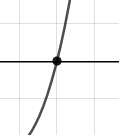
\includegraphics[width = 0.3\textwidth]{../Figures/polyZeroBehaviorCopyDC.png}\end{multicols}\item None of the above.
\end{enumerate} }
\litem{
Which of the following equations \textit{could} be of the graph presented below?
\begin{center}
    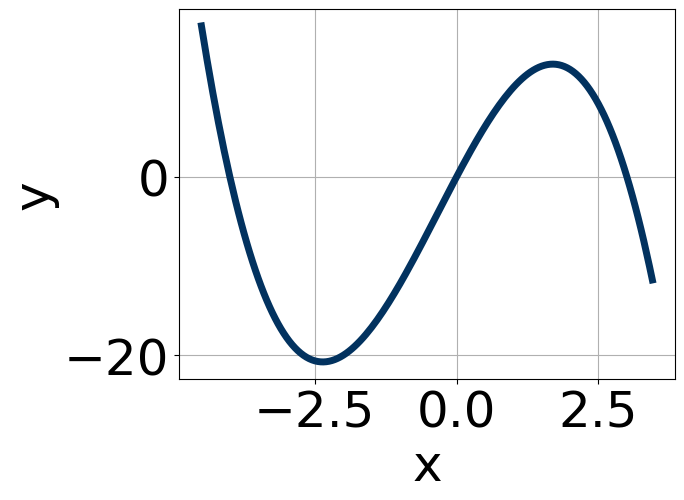
\includegraphics[width=0.5\textwidth]{../Figures/polyGraphToFunctionCopyC.png}
\end{center}
\begin{enumerate}[label=\Alph*.]
\item \( -17x^{9} (x + 4)^{6} (x - 3)^{11} \)
\item \( -19x^{10} (x + 4)^{6} (x - 3)^{7} \)
\item \( -8x^{9} (x + 4)^{9} (x - 3)^{7} \)
\item \( 13x^{11} (x + 4)^{7} (x - 3)^{7} \)
\item \( 16x^{7} (x + 4)^{10} (x - 3)^{9} \)

\end{enumerate} }
\litem{
Describe the end behavior of the polynomial below.\[ f(x) = -3(x + 5)^{5}(x - 5)^{8}(x + 9)^{2}(x - 9)^{3} \]\begin{enumerate}[label=\Alph*.]
\begin{multicols}{2}\item 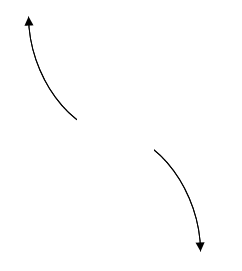
\includegraphics[width = 0.3\textwidth]{../Figures/polyEndBehaviorAC.png}\item 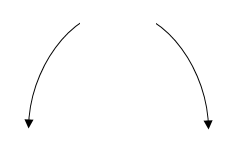
\includegraphics[width = 0.3\textwidth]{../Figures/polyEndBehaviorBC.png}\item 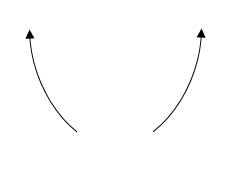
\includegraphics[width = 0.3\textwidth]{../Figures/polyEndBehaviorCC.png}\item 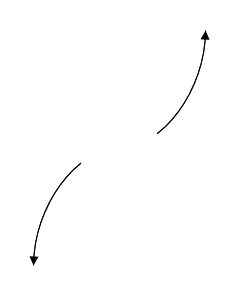
\includegraphics[width = 0.3\textwidth]{../Figures/polyEndBehaviorDC.png}\end{multicols}\item None of the above.
\end{enumerate} }
\litem{
Construct the lowest-degree polynomial given the zeros below. Then, choose the intervals that contain the coefficients of the polynomial in the form $x^3+bx^2+cx+d$.\[ 4 - 3 i \text{ and } -1 \]\begin{enumerate}[label=\Alph*.]
\item \( b \in [6, 11], c \in [16, 18], \text{ and } d \in [-26, -24] \)
\item \( b \in [-9, -4], c \in [16, 18], \text{ and } d \in [20, 28] \)
\item \( b \in [-2, 6], c \in [-4, -2], \text{ and } d \in [-4, -1] \)
\item \( b \in [-2, 6], c \in [3, 5], \text{ and } d \in [-1, 8] \)
\item \( \text{None of the above.} \)

\end{enumerate} }
\litem{
Construct the lowest-degree polynomial given the zeros below. Then, choose the intervals that contain the coefficients of the polynomial in the form $ax^3+bx^2+cx+d$.\[ \frac{-2}{3}, \frac{-1}{4}, \text{ and } \frac{7}{4} \]\begin{enumerate}[label=\Alph*.]
\item \( a \in [44, 54], b \in [-110, -98], c \in [21, 29], \text{ and } d \in [9, 22] \)
\item \( a \in [44, 54], b \in [-41, -35], c \in [-74, -64], \text{ and } d \in [-15, -11] \)
\item \( a \in [44, 54], b \in [-41, -35], c \in [-74, -64], \text{ and } d \in [9, 22] \)
\item \( a \in [44, 54], b \in [-134, -124], c \in [85, 86], \text{ and } d \in [-15, -11] \)
\item \( a \in [44, 54], b \in [40, 42], c \in [-74, -64], \text{ and } d \in [9, 22] \)

\end{enumerate} }
\litem{
Describe the end behavior of the polynomial below.\[ f(x) = 3(x - 3)^{2}(x + 3)^{7}(x + 9)^{5}(x - 9)^{7} \]\begin{enumerate}[label=\Alph*.]
\begin{multicols}{2}\item 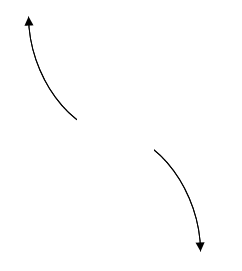
\includegraphics[width = 0.3\textwidth]{../Figures/polyEndBehaviorCopyAC.png}\item 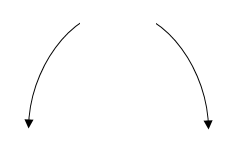
\includegraphics[width = 0.3\textwidth]{../Figures/polyEndBehaviorCopyBC.png}\item 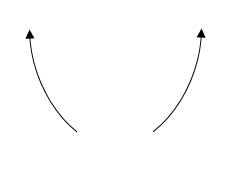
\includegraphics[width = 0.3\textwidth]{../Figures/polyEndBehaviorCopyCC.png}\item 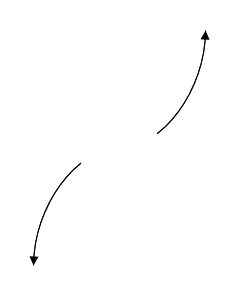
\includegraphics[width = 0.3\textwidth]{../Figures/polyEndBehaviorCopyDC.png}\end{multicols}\item None of the above.
\end{enumerate} }
\litem{
Which of the following equations \textit{could} be of the graph presented below?
\begin{center}
    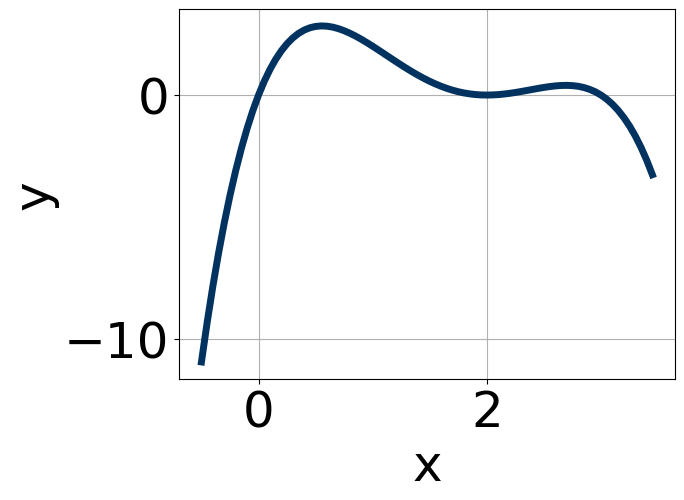
\includegraphics[width=0.5\textwidth]{../Figures/polyGraphToFunctionC.png}
\end{center}
\begin{enumerate}[label=\Alph*.]
\item \( 17(x - 1)^{10} (x - 3)^{6} (x + 4)^{11} \)
\item \( -20(x - 1)^{10} (x - 3)^{11} (x + 4)^{11} \)
\item \( 4(x - 1)^{8} (x - 3)^{11} (x + 4)^{5} \)
\item \( -20(x - 1)^{11} (x - 3)^{5} (x + 4)^{5} \)
\item \( 4(x - 1)^{11} (x - 3)^{11} (x + 4)^{9} \)

\end{enumerate} }
\end{enumerate}

\end{document}